% Ch1Introduction.tex

\chapter[Introduction]{Introduction}
\label{cha:cha1Introduction}
\pagenumbering{arabic}
%=============
\section{Motivation and Overview}
Over the last two decades, rapid decline in frog populations, which is regarded as one of the most critical danger to the global biodiversity, has been spotted worldwide. The causes for this decline are many, but an emerging disease called \textit{chytridiomycosis}   \citep{mutschmann2015chytridiomycosis} and global climate change \citep{carey2003climate} are thought as the biggest threats. On the one hand frog populations are declining rapidly, but on the other, frogs are greatly important to the Earth's ecosystem. For instance, frogs are an integral part of the food web, and are often considered as a valuable indicator for their sensitivity to the environmental change \citep{boll2013amphibians}. Therefore, it is becoming ever more important to develop better tools for frog monitoring. 
In the field, frogs are often much easier to be heard than seen (Figure~\ref{fig:Ch1_frogs}). 


\begin{figure*}[htb!]
\centering
      \begin{subfigure}[b]{0.5\textwidth}
           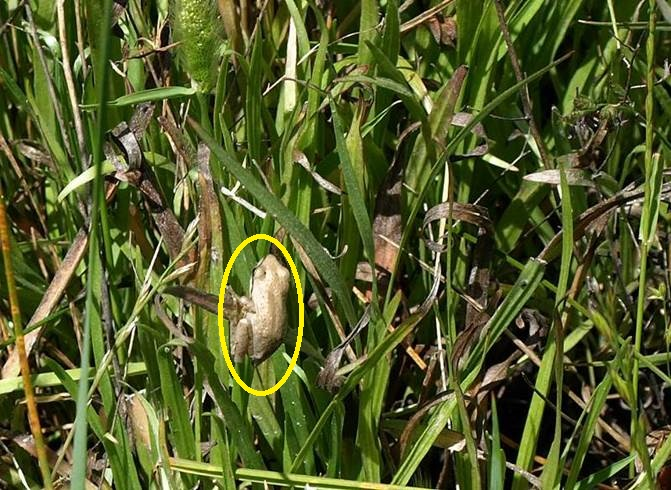
\includegraphics[width=1\textwidth,height=0.75\textwidth]{image/Ch1/unseen_frog_1.jpg}
    \end{subfigure}%
	~~
	      \begin{subfigure}[b]{0.5\textwidth}
           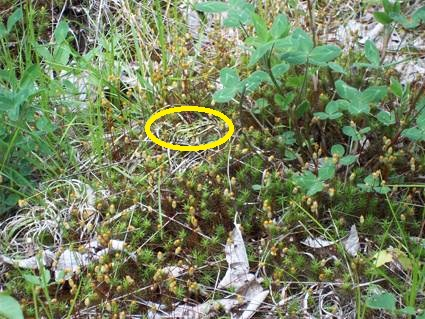
\includegraphics[width=1\textwidth,height=0.75\textwidth]{image/Ch1/unseen_frog_2.jpg}
    \end{subfigure}%
\caption[Photos of frogs]{Photos of frogs to indicate that frogs are difficult to be found in the field}
\label{fig:Ch1_frogs}       % Give a unique label
\end{figure*}


Also frog vocalisations are often employed for most communications, which offer a possible way to study and evaluate frogs by detecting species-specific calls \citep{dorcas2009auditory}. Traditional methods require ecologists and volunteers to physically visit sites for acoustic data analysis, which are costly and time-consuming. 
Although traditional methods can provide an accurate measure of daytime species and richness, the scale limitation in both spatial and temporal domains is unavoidable. To address this limitation, recent advances in acoustic sensors provide a way to automatically survey vocal animals (such as frogs). Deploying acoustic sensors in the field, frog vocalisations can then be automatically collected. Compared to the manual point-counting method, sensors can greatly extend the survey into larger spatial and temporal scales, and generate large volumes of acoustic data that needs to be analysed. Consequently, enabling automatic species identification in acoustic data has become increasingly important. 

%In contrast, recent advances in acoustic sensors provide a novel method to survey vocalising animals such as frogs. Once acoustic sensors are successfully installed in the field, acoustic data can be automatically collected at large spatial and temporal scales. For each acoustic sensor, 
%several gigabytes of compressed audio data can be generated per day, and large volumes of raw acoustic data have been collected. Enabling automated species classification in acoustic data has become very important to gain insights about frogs.


To build an accurate and robust frog call classification system for environmental recordings, two major challenges must be faced:

\begin{enumerate}
\item  Compared to commercial recordings which are collected in constrained environment with a directional microphone, environmental recordings tend to be noisy. Very often the desired signal (frog call) is weak, and there are other overlapping signals such as bird calls and insect calls over frog calls. Therefore, features used for classifying frogs in environment recordings must have a good anti-noise ability.


\item  Most environmental recordings contain multiple frog species in an individual recording (Figure.~\ref{fig:label}), which is different from recordings used in previous studies (one species per recording). The classification framework used for classifying frog species in environmental recordings must be able to predict multiple labels for one individual recording.



\end{enumerate}
 


\begin{figure}[htb!]
\centering
    \begin{subfigure}[b]{\textwidth}
           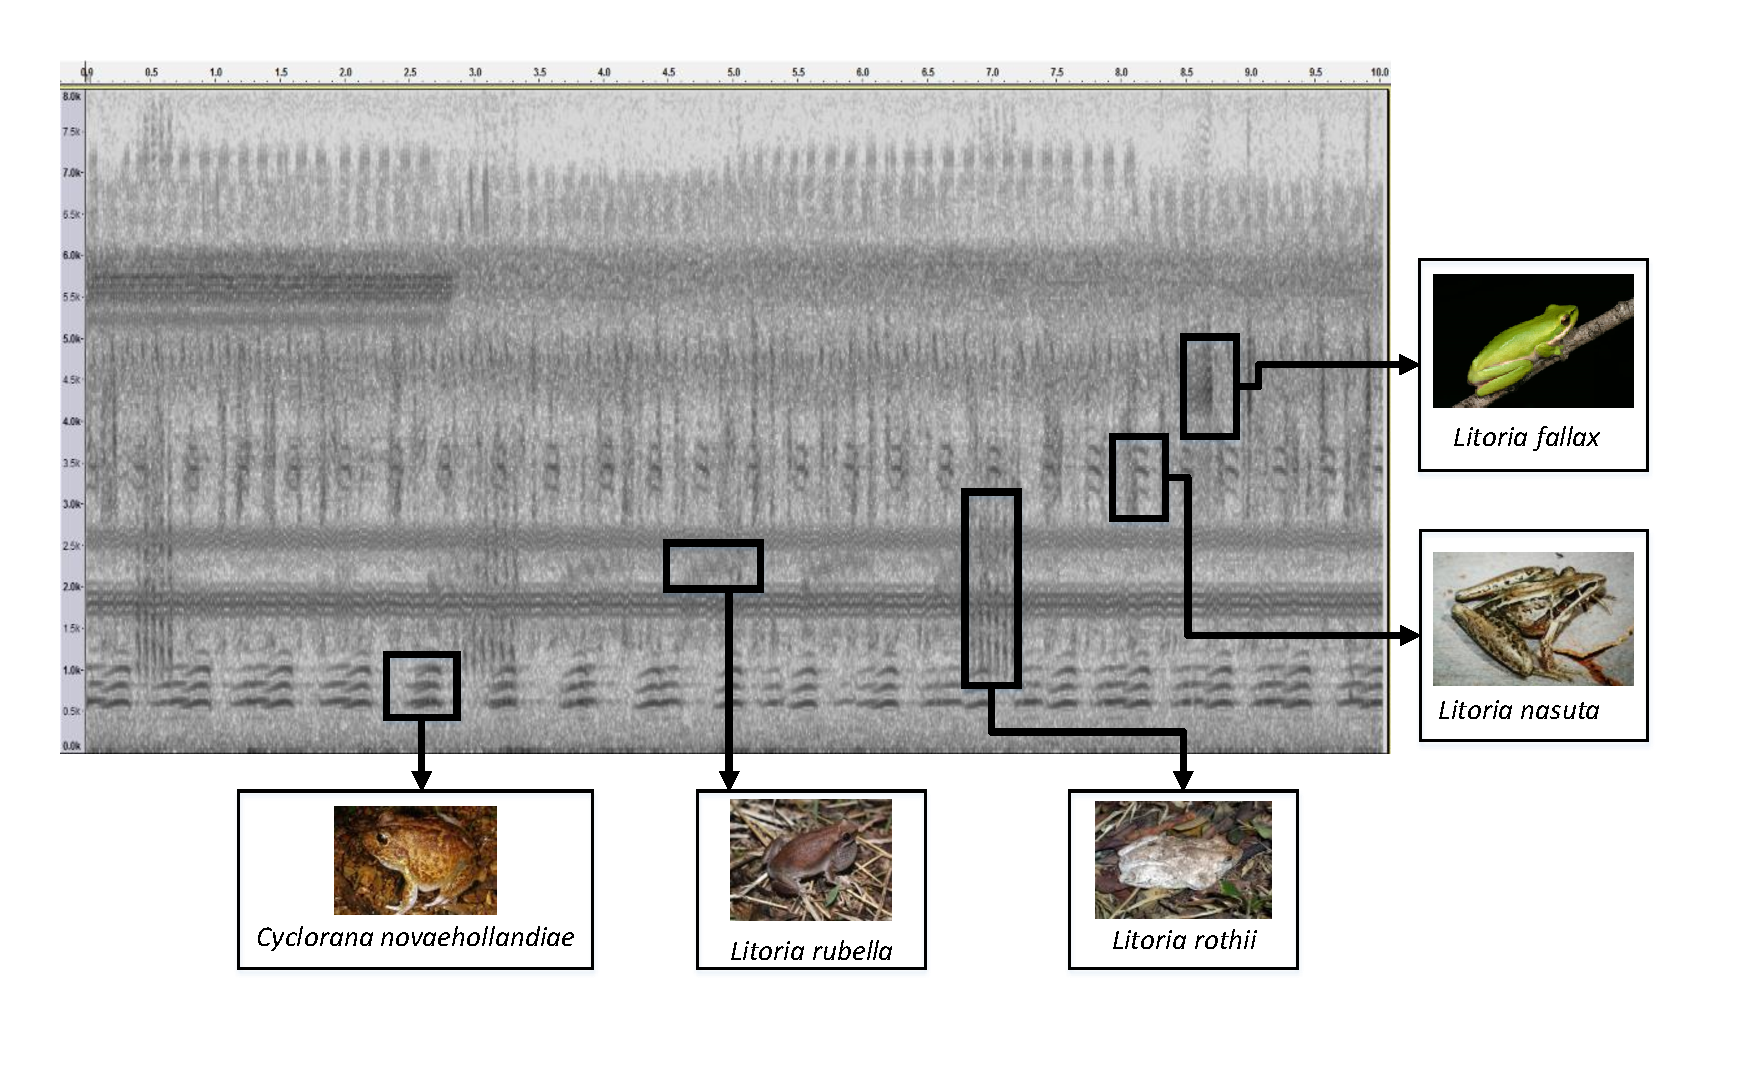
\includegraphics[width=1\textwidth]{image/LR/label.pdf}
    \end{subfigure}%
\caption[An example of collected recording]{An example of collected recording with multiple simultaneously vocalising frog species. Five frog species exist in this 10-second recording: \textit{Cyclorana novaehollandiae}, \textit{Litoria rubella}, \textit{Litoria nasuta}, \textit{Litoria rothii}, and \textit{Litoria fallax}.}
\label{fig:label}       
\end{figure}




%audio data, which are collected using acoustic sensors in the field, tends to be noisy. Very often the desired signal (frog call) is weak, and there are other overlapping signals such as bird calls/insect calls over frog calls. Furthermore, different frog species tend to call together to make a chorus. All those characteristics pose a big challenge to performing automatic classification of frog species in audio data collected by sensors. 


\section{Scope of PhD}
The broad scope of this PhD research is to address the aforementioned two  major challenges, which could pave a way to successful classification of frog species in environmental recordings. The outcome of the research is of benefit to many applications of bioacoustics.

In recent times, various frog call classification methods have been proposed, but the recordings used often have a high SNR and contain only one frog species. Our first experiment aims to propose a fused feature set to further improve the performance of classifying frog species in high SNR recordings. The second experiment moves to develop a novel cepstral feature that can classify frog species in low SNR recordings.
However, those two experiments assume that each individual recording contain only one frog species. In the third experiment, a novel MIML classification framework is proposed to classify frog species in low SNR recordings with multiple frog species. The last experiment is to further improve the performance for classifying frog species in low SNR recordings with multiple frog species, where a novel ML classification framework is used.



\section{Thesis Structure}

This thesis is organised in the manner outlined in Figure~\ref{fig:mainchapters}

\begin{figure}[htb!]
\centering
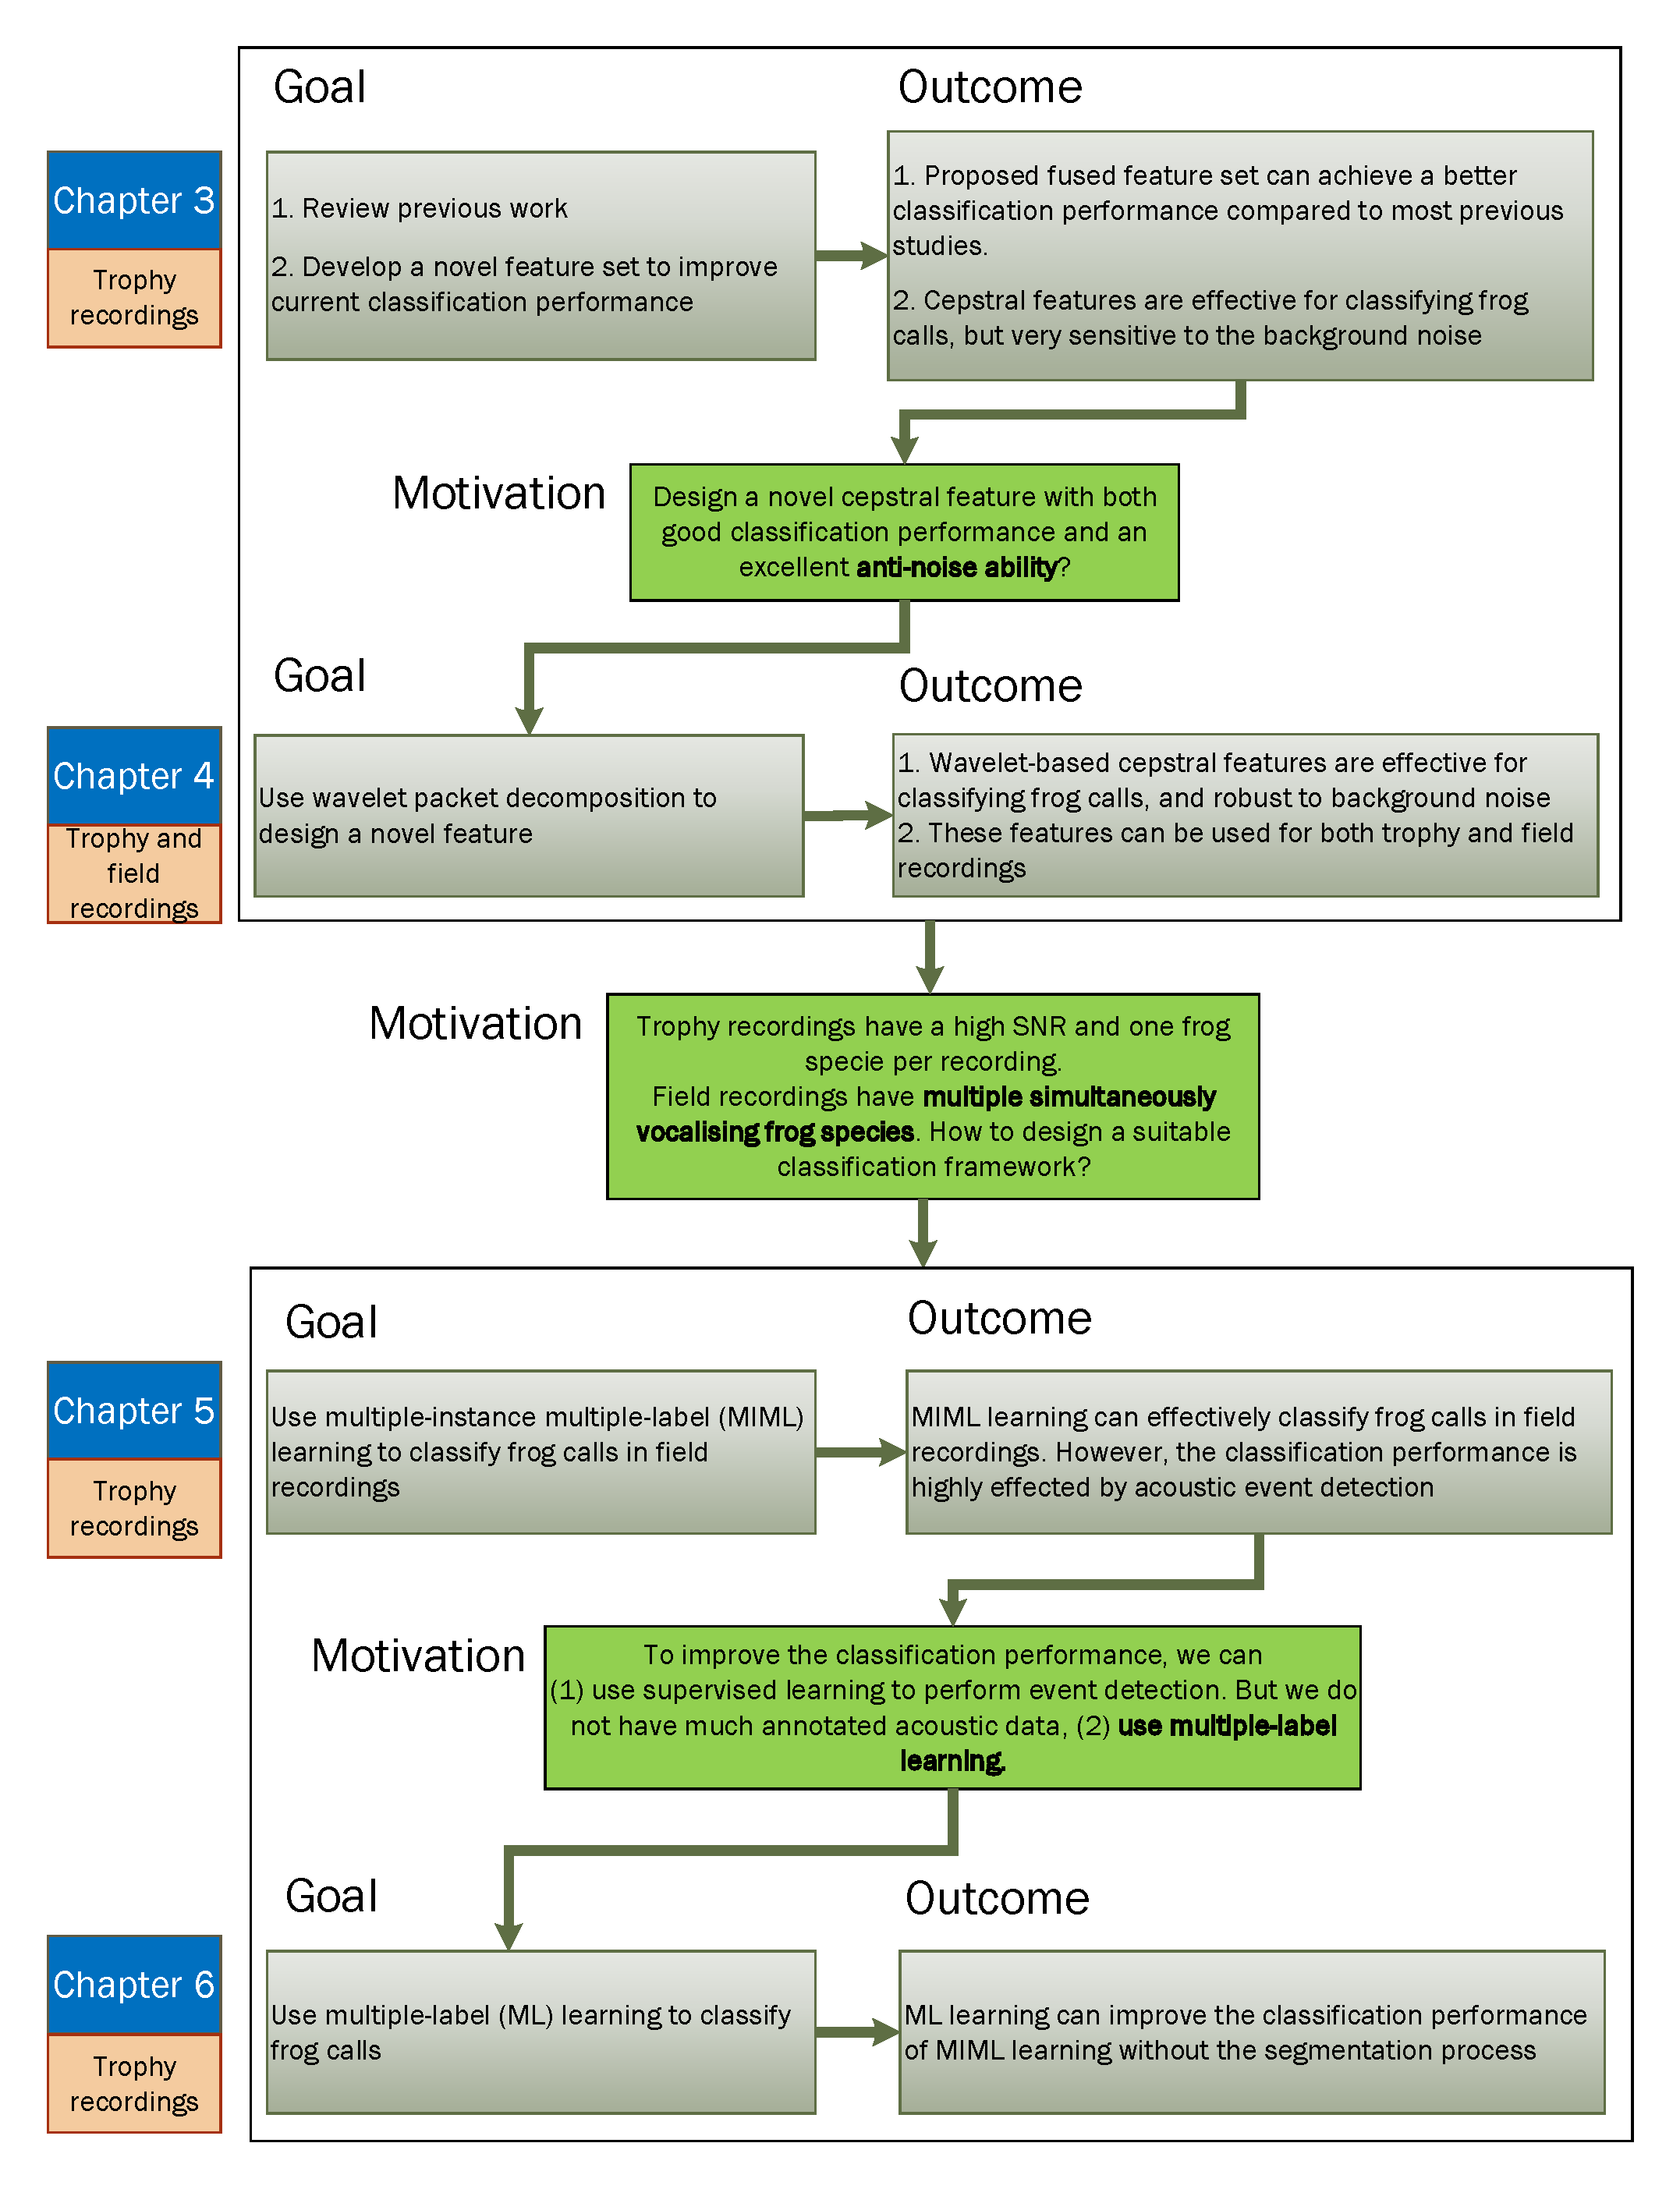
\includegraphics[width=\textwidth]{image/Ch1/structure_chapters.pdf}
\caption[Structure of the four main chapters of this thesis]{Structure of the four main chapters of this thesis}
\label{fig:mainchapters}
\end{figure}



\begin{itemize}
%\item  Chapter \ref{cha:cha1Introduction} provides a brief introduction to the problem of "Acoustic classification of Australian frogs for ecosystem surveys". The background and motivation are first discussed. Then five basic concepts related to frog call classification are presented to lay the foundation for this research: environmental audio data, audio data analysis, frog call structure, acoustic event and background noise, and frog call classification system. Next, research problems and questions, aims and objectives, significance and contributions are presented based on those five basic concepts. To be specific, there are three main objectives in this thesis. The remaining chapters are organised in the order of addressing those three objectives.

\item Chapter \ref{cha:cha2LiteratureReview} reviews the significant and latest literature of frog call classification using machine learning techniques. Three main parts of a frog call classification system are discussed: syllable segmentation, feature extraction, and classification. 
In addition, evaluation metrics and previous experimental results are presented. This chapter intends to provide a foundation for the research problem and necessary information about the state-of-the-art development of frog call classification. Furthermore, the research gap is identified, which points out the potential research direction.


\item Chapter \ref{cha:cha4EnhancedFeature} develops a fused feature set for further improving the performance of frog call classification using high SNR recordings. A fusion of temporal, perceptual, and cepstral features is proposed for frog call classification. The classification performance of five machine learning algorithms are studied with the fused feature set. 

%This chapter aims to (1) review previous features used for frog call classification and develop a better feature set; (2) explore those previous features and study which can be adapted from high SNR recordings to low SNR recordings.


\item  Chapter \ref{cha:cha5WaveletFeature} investigates WPD for extracting a novel cepstral feature. An adaptive frequency scale is first generated by applying k-means clustering to dominant frequencies of the training dataset.
Then, adaptive frequency scaled WPD is used for calculating cepstral features. Two other cepstral features are used for the comparison. Two machine learning algorithms are used for the classification.


%discusses wavelet analysis for frog call classification. According to the conclusion from Chapter \ref{cha:cha4EnhancedFeature}, it is found that a ceptral feature can achieve higher classification accuracy compared with temporal and perceptual features but it is very sensitive to the background noise. Consequently, in this research, a novel cepstral feature has been designed with wavelet packet decomposition that has both high classification performance and a good anti-noise ability. It is because this research will move to low SNR recordings from high SNR recordings, rather than only focusing on the low SNR recordings.


\item  Chapter \ref{cha:cha6MIML} discusses the limitations of traditional SISL classification framework for classify frog species in low SNR recordings, and proposed a novel MIML classification framework to classify frog species in low SNR recordings with multiple frog species. A novel AED method is developed for frog syllable segmentation. Three MIML classifiers are combined with features extracted from segmented syllables to perform the classification.


 

%MIML learning is presented in this chapter. A MIML classification framework is adopted for studying frogs. A previous study of studying birds used a supervised learning algorithm to segment frog syllables, but needs lots of annotated data. However, there are few annotated frog recordings in this study. An unsupervised learning method is therefore developed to segment syllables, which is named \textit{acoustic event detection} (AED). Then, three MIML classifiers are evaluated with constructed features using a bagging generator. The proposed MIML classification framework can classify multiple frog species in low SNR recordings, but the classification performance is highly affected by the results of AED. Although our AED methods achieves better results compared with previous AED methods, the results still need to be further improved.


\item  Chapter \ref{cha:cha7ML} investigates the shortcomings of the MIML classification framework, and introduces ML learning for classify frog species in low SNR recordings with multiple frog species. Subsequently, three global features are calculated without the segmentation process.  Four ML classifiers are then used for the classification with various combined feature sets.

\item Chapter \ref{cha:cha8Application} applies the ML classification for the long-term monitoring of frog calling activity and species richness.
Both frog calling activity and species richness over three months are estimated. Frog species richness of three different sites are compared.  
The correlation between frog calling activity/species richness and weather variables (mean temperature and rainfall) are investigated. 


%Chapter \ref{cha:cha6MIML} demonstrates that classification performance is highly affected by AED results. In this chapter, we use ML learning to study low SNR recordings with multiple simultaneously vocalising frog species without the segmentation process. 
%Two experiments are conducted in this chapter. The first is to estimate the frog calling activity using the AED. The second is to estimate the frog species richness using the global feature sets, where the feature sets are modified from  those features used in Chapter \ref{cha:cha4EnhancedFeature}. Furthermore, both frog calling activity and species richness over three months are estimated using the field recordings.
%The correlation between frog calling activity/species richness and weather variables (mean temperature and rainfall) are studied.


\item  Chapter \ref{cha:cha8Conclusions} summarises and concludes the thesis, and identifies the achievements.

\end{itemize}

\section{Original contributions}
This research makes important contributions to the domains of syllable segmentation, feature extraction, and classification. Specifically, this research proposes a novel AED to segment frog syllables in low SNR recordings. For further improving the classification performance using high SNR recordings, a fused feature set from temporal, perceptual, and cepstral features is constructed. To increase the anti-noise ability of cepstral features, a novel cepstral feature via adaptive frequency scaled WPD is developed. Moreover, two classification frameworks, MIML classification and ML classification, are used to cope with low SNR recording including multiple frog species.

\begin{enumerate}

\item Most previous studies test the proposed frog call classification methods using high SNR recordings, and each recording has only one frog species. The first experiment of this thesis aims to further improve the classification performance using high SNR recordings. A novel feature fusion using temporal, perceptual, and cepstral features is proposed for the classification. To reduce the bias of syllable segmentation, Gaussian filtering is selectively used to remove the temporal gap within one syllable. For various fused feature sets, five machine learning algorithms are used for the classification. Experimental results on high SNR recordings show that our proposed feature set outperforms other widely used feature sets for classifying frog calls. 

This research has led to one ISSNIP conference paper, one Applied Acoustic  journal article.

\item Since most environmental recordings have a low SNR, the anti-noise ability is critical for achieving a good classification performance. Previous studies demonstrate that cepstral features used for classifying high SNR recordings often have a high classification accuracy. However, those cepstral features are very sensitive to the background noise.
A novel cepstral feature is proposed via adaptive frequency scaled WPD for classifying frog species in low SNR recordings. Here, the adaptive frequency scale is generated by applying k-means clustering to the dominant frequencies of training dataset. Previous studies have shown that dominant frequencies of most different frog species are different. Generating a frequency scale that can best describe the frequency distribution of different frog species can greatly the discriminability of extracted features. Experimental results show that our proposed cepstral feature not only outperform other cepstral features but also has a better anti-noise ability.

This research has led to one ICISP conference paper, one IEEE e-science conference paper, and one Ecological Informatics journal article.

\item Since most environmental recordings contain multiple frog species of one individual recording, the MIML classification framework is a natural fit for acoustic data of frog calls, and enables the classification of multiple simultaneously vocalising frog species. A novel AED method is proposed for the segmentation of frog syllables in low SNR recordings with limited annotated data. Compared to other AED methods, our proposed AED method can achieve the best syllable segmentation results. For each segmented frog syllable, low-level features are calculated. Three MIML classifiers are then used for the classification with various feature sets build from low-level features.
Experimental results demonstrate that our proposed MIML classification framework can achieve a better classification performance than the SISL classification framework.

This research has led to one ICISP conference paper.

\item For the MIML classification, the results are highly affected by the AED results. To further improve the classification performance, one solution is to prepare large volumes of annotated acoustic data and apply supervised learning algorithms for improving segmentation results. Another is to used a different framework without the need of syllable segmentation. This thesis examines the latter option and proposes a ML classification framework to classify multiple simultaneously vocalising frog species. Three global features are first extracted from each individual recordings: LPCs, MFCCs, and PWSCCs. Then a novel feature set using LPCs and multi-stage PWSCCs is used for the ML classification.
Experimental results show that ML classification results outperform MIML classification results. 

This research has led to a ICCS conference paper.


\end{enumerate}
 




\section{Publications}

{\textbf{Journal Articles}}
\begin{enumerate} 

\item  \textbf{Xie, Jie}, Towsey, Michael, Zhang, Jinglan, and Roe, Paul, Frog call classification based on enhanced features and machine learning algorithms, Applied Acoustics, Volume 113, June 2016, pp. 193-201.

This work corresponds to Chapter \ref{cha:cha4EnhancedFeature} in this thesis, which presents a fused feature set for frog call classification in high SNR recordings.

\item	\textbf{Xie, Jie}, Towsey, Michael, Zhang, Jinglan, and Roe, Paul (2016) Adaptive frequency scaled wavelet packet decomposition for frog call classification.  Ecological Informatics, Volume 32, pp. 134-144.

This work corresponds to Chapter \ref{cha:cha5WaveletFeature} in this thesis, which develops a novel cepstral feature for frog call classification in low SNR recordings.



\item	Zhang Liang, Towsey Michael, \textbf{Xie Jie}, Zhang Jinglan, Roe Paul,  Using multi-label classification for acoustic pattern detection and assisting bird species surveys, Applied Acoustics, Volume 110, September 2016, Pages 91-98.

\item \textbf{Xie, Jie}, Towsey, Michael, Zhang, Jinglan, and Roe, Paul, Frog call classification: a survey, Artificial Intelligence Review (\textbf{Under review})


This work corresponds to Chapter \ref{cha:cha2LiteratureReview} in this thesis, which reviewed the extant literature on frog call classification.



\end{enumerate}

{ \textbf{Conference Papers}}
\begin{enumerate} 

\item \textbf{Xie, Jie}, Michael Towsey, Jinglan Zhang, Paul Roe, Detecting Frog Calling Activity Based on Acoustic Event Detection and Multi-label Learning, Procedia Computer Science, Volume 80, 2016, Pages 627-638.
 
 
This work corresponds to Chapter \ref{cha:cha6MIML} in this thesis, which applied ML learning for frog call classification. 
 
 
\item \textbf{Xie, Jie}, Towsey, Michael, Zhang, Liang, Yasumiba, Kiyomi and Schwarzkopf, Lin,  Zhang, Jinglan, and Roe, Paul. Multiple-Instance Multiple-Label Learning for the Classification of Frog Calls with Acoustic Event Detection. International Conference on Image and Signal Processing. Springer International Publishing, 2016, pp 222-230.
 
This work corresponds to Chapter \ref{cha:cha7ML} in this thesis, which applies MIML learning for frog call classification. 
 
 
 
\item \textbf{Xie, Jie}, Towsey, Michael, Zhang, Liang, Zhang, Jinglan, and Roe, Paul, Feature Extraction Based on Bandpass Filtering for Frog Call Classification, International Conference on Image and Signal Processing, Springer International Publishing, 2016, pp 231-239.


\item	\textbf{Xie, Jie}, Towsey, Michael, Truskinger, Anthony, Eichinski, Philip, Zhang, Jinglan, and Roe, Paul (2015) Acoustic classification of Australian anurans using syllable features. In 2015 IEEE Tenth International Conference on Intelligent Sensors, Sensor Networks and Information Processing (ISSNIP), IEEE, Singapore, pp. 1-6.

\item	\textbf{Xie, Jie}, Towsey, Michael, Yasumiba, Kiyomi, Zhang, Jinglan, and Roe, Paul (2015) Detection of anuran calling activity in long field recordings for bio-acoustic monitoring. In 2015 IEEE Tenth International Conference on Intelligent Sensors, Sensor Networks and Information Processing (ISSNIP), IEEE, Singapore, pp. 1-6.



\item	\textbf{Xie, Jie}, Towsey, Michael, Zhang, Jinglan, and Roe, Paul (2015) Image processing and classification procedure for the analysis of Australian frog vocalisations. InProceedings of the 2nd International Workshop on Environmental Multimedia Retrieval, ACM, Shanghai, China, pp. 15-20.


\item	\textbf{Xie, Jie}, Towsey, Michael, Zhang, Jinglan, Dong, Xueyan, and Roe, Paul (2015)Application of image processing techniques for frog call classification. In IEEE International Conference on Image Processing (ICIP 2015), 27-30 September 2015, Québec City, Canada.

\item	\textbf{Xie, Jie}, Towsey, Michael, Eichinski, Philip, Zhang, Jinglan, and Roe, Paul (2015)Acoustic feature extraction using perceptual wavelet packet decomposition for frog call classification. In 2015 IEEE 11th International Conference on e-Science (e-Science), IEEE, Munich, Germany, pp. 237-242.

\item	\textbf{Xie, Jie}, Zhang, Jinglan and Roe, Paul,  “Discovering acoustic feature extraction and selection algorithms for frog vocalization monitoring with machine learning techniques”, 2015 Annual Conference of the Ecological Society of Australia. (Abstract accepted for poster presentation) 

\item	\textbf{Xie, Jie}, Zhang, Jinglan, and Roe, Paul (2015) Acoustic features for hierarchical classification of Australian frog calls. In 10th International Conference on Information, Communications and Signal Processing, 2-4 December 2015, Singapore.

\item	Dong, Xueyan, \textbf{Xie, Jie}, Towsey, Michael, Zhang, Jinglan, and Roe, Paul (2015)Generalised features for bird vocalisation retrieval in acoustic recordings. In IEEE International Workshop on Multimedia Signal Processing, 19-21 October 2015, Xiamen, China.

\end{enumerate} 
%===============
%\section{Basic concepts} 
%This section presents some basic concepts to better describe the research problem and questions, aims and objectives, significance and contributions.
%
%\section{Commercial recordings VS Environmental recordings}
%In this thesis, recordings are derived from two sources: David Stewart's commercial recordings \citep{CD} (high SNR and one species per recording) and James Cook University's environmental recordings (JCU) \footnote{All the recordings can be requested and obtained from our group website: https://www.ecosounds.org/} (low SNR and multiple species per recording). Here, commercial recordings often have a high SNR and each individual recording has only one frog species. In contrast, JCU recordings often have a low SNR, and most of them contain multiple frog species. 
%The SNR of commercial recordings and environmental recordings are listed in Table~\ref{tab:wav_spec_cd} and Table~\ref{tab:JCU_para}. 
%%Since the power of signal and background noise in this study varies from recording to recording and call to call within the recording, Tables~\ref{tab:CI_CD} and \ref{tab:CI_JCU} show the confidence intervals of high and low SNR recordings for the power of signal and noise. 
%
%
%Since almost all prior work for frog call classification has an assumption that each individual recording contains only one frog species. To make a direct comparison with those previous studies, two experiments are designed using high SNR recordings. 
%However, most field recordings contain multiple simultaneously vocalising frog species, we therefore propose two classification frameworks to study environmental recordings (JCU recordings): MIML classification and ML classification. 





%First, a fused feature set is developed for classifying frog species in high SNR recordings, and the performance of this fused feature set outperforms other compared features sets. The second is to develop a novel cepstral feature to classify frog species in high SNR recordings. The classification results show that our proposed feature not only achieves the best classification accuracy but also has a good anti-noise ability compared with other cepstral features.

%First, MIML learning is used to classify frog species in low SNR recordings with AED. Experimental results indicate that the use of MIML learning can successfully classify multiple frog species in low SNR recordings. 
%
%To ease the limitaion of AED,
%
%
%
% Chapters \ref{cha:cha6MIML} and \ref{cha:cha7ML} focus on the investigation of JCU recordings, which is the real situation for most environmental recordings. 

%
%\end{itemize}


%Compared to audio data collected using a directional microphone to record a single frog's calls (David Stewart$’$s CD), environmental recordings are normally collected under unconstrained noisy conditions (such as JCU recordings). Consequently, the noise and variability issues need to be considered when coping with environmental audio data. 
%In terms of the background noise, there are a wide variety of non-biological noises and a variety of animal sounds in environmental recordings. These non-biological noises often come from different sources: rain, wind, human activities (e.g. traffic noise). Besides non-biological noises, many competitive animal sounds (e.g. birds when we are interested in frogs) are also recorded in the environmental recordings. 


%The SNR is calculated as follows:
%
%\begin{equation}
%SNR=10*log_{10}(\frac{\sum_{i=m}^{m+L}S_{i}^2}{\sum_{j=n}^{n+L}N_{j}^2})
%\end{equation}
%where $L$ is the length of the signal and noise used for calculating SNR, and set at 6000 samples here, $n$ and $m$ are manual selected start location in the waveform for noise and signal, respectively. 





%The calculation of confidence interval is defined as follows:
%
%\begin{equation}
%CI=\mu \pm Z*\frac{\sigma}{\sqrt{L}}
%\end{equation}
%where $\mu$ and $\sigma$ are the mean and standard deviation, respectively, $Z$ is the upper $\frac{(1-C)}{2}$ critical value for the standard normal distribution, $C$ is the confidence level, and set at 0.95.



%In the case of variability, it is produced in many aspects: call structure between species, population of one specific species, time and season changes. All those noises and variabilities make it challenging to develop a robust frog call classification system. 





%
%\subsection{Audio data analysis}
%Audio data is usually considered as a mono-dimensional signal. To ease the tasks of understanding, comparison, modification, and re-synthesis of signals \citep{rocchesso2003introduction}, audio data analysis is often developed to find the major features representing the time-varying audio data. Many application areas of audio data analysis have been identified: speech processing, mechanical signal processing, bioacoustics analysis, etc. The two most important audio data analysis techniques are Short-time Fourier Transform (STFT) and Linear Predictive Coding (LPC). STFT is a Fourier-related transform, which determines the sinusoidal frequency and phase content of local sections of a signal as it changes over time \citep{allen1997short}. LPC is mostly used to represent the spectral envelope of audio data based on the information of a linear predictive model \citep{deng2003speech}. After STFT, the audio data is transformed into its two dimensional representation (spectrogram), which is widely used for most bioacoustic analysis for its flexible implementation and good applicability.
%An example of a spectrogram of frog calls derived from a field recording is shown in Figure~\ref{fig:Ch1_spectrogram}.
%
%\begin{figure}[htb!]
%\centering
%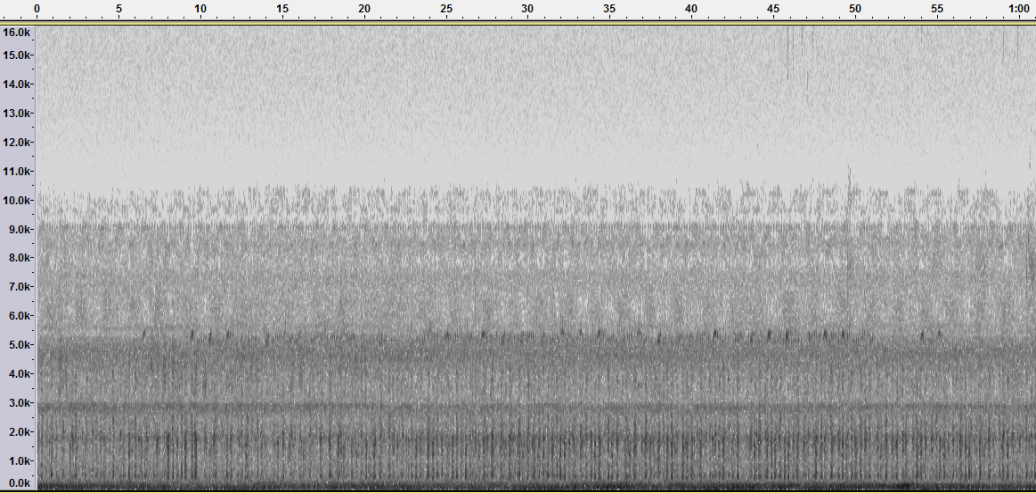
\includegraphics[width=\textwidth]{image/Ch1/spectrogram_example.png}
%\caption[An example of a spectrogram of environmental recording]{An example of spectrogram of environmental recording. The x-axis is time (seconds); the y-axis is frequency (kHz). The spectrogram is generated from a one-minute recording collected in Townsville, Queensland, on around 11.50 pm February 03 2013; the frog species in this recording is \textit{Litoria caerulea}}
%\label{fig:Ch1_spectrogram}
%\end{figure}
%
%
%
%
%
%%===================
%\subsection{Frog call structure}
%In contrast to the hierarchical structure of bird calls, frog calls have a relatively simple call structure \citep{somervuo2006parametric}. The frog vocalisation structure mainly has two ingredients: call and syllable. A frog call is normally made up of several syllables (Figure~\ref{fig:Ch1_spec_mark}).
%
%\begin{figure}[htb!]
%\centering
%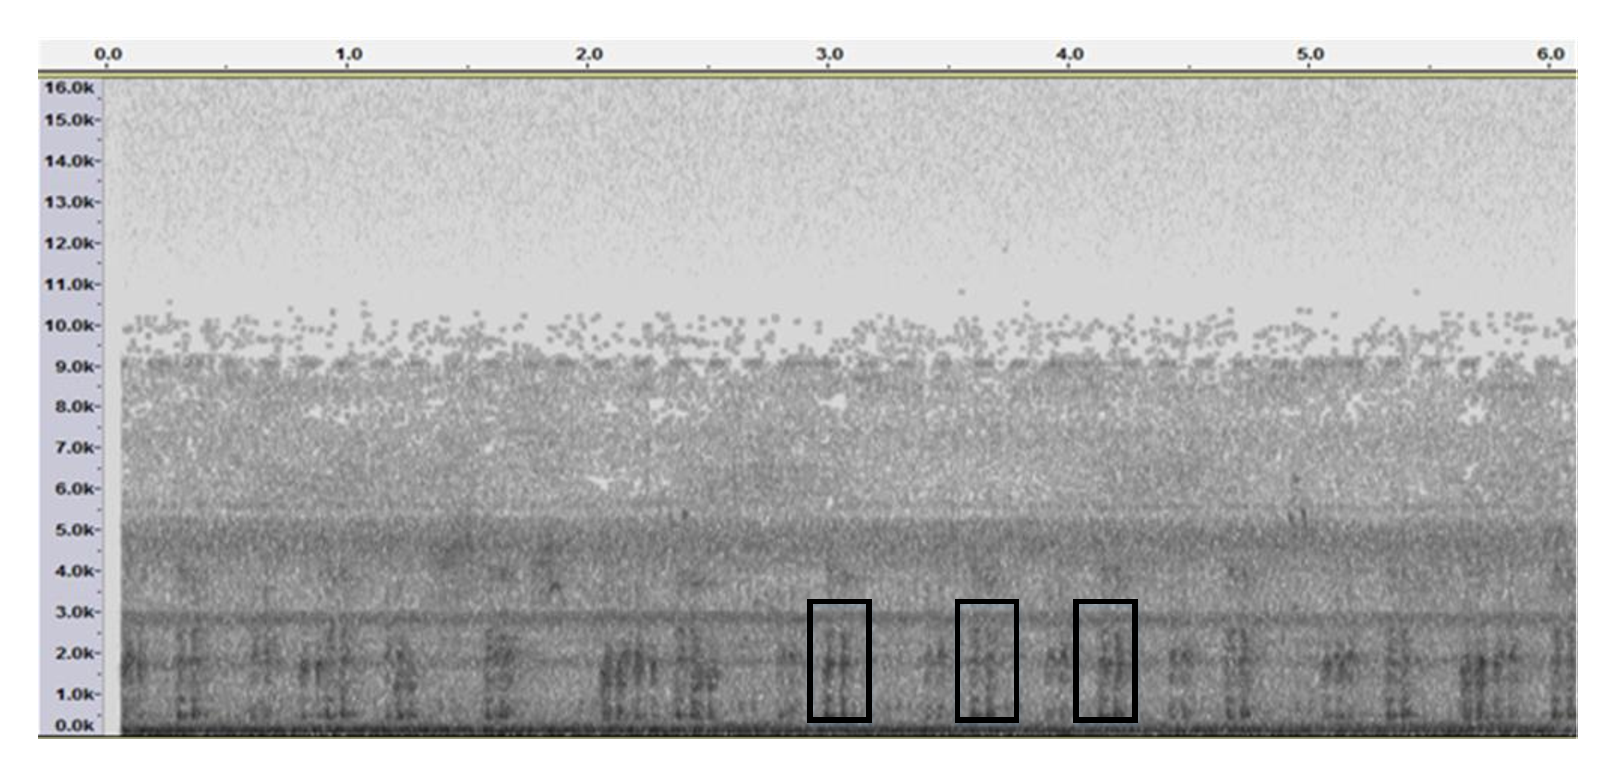
\includegraphics[width=\textwidth]{image/Ch1/spectrogram_mark.pdf}
%\caption[Spectrogram of \textit{Litoria caerulea}]{Spectrogram of \textit{Litoria caerulea}, three syllable of \textit{Litoria caerulea} are annotated with one black rectangle, respectively.}
%\label{fig:Ch1_spec_mark}
%\end{figure}
%
%
%One syllable is basically a sound that a frog produces with a single blow of air from the lungs \citep{huang2009frog}. For frog call classification, an elementary unit is one syllable. 
%To get an intuitive sense of the frog call structure, examples of different frog species in both waveform and spectrogram are shown in Table~\ref{tab:wav_spec_cd} and Table~\ref{tab:JCU_para}. For the waveform, x-axis and y-axis represent time and amplitude scales, respectively. The x-axis and y-axis of the spectrogram represent the time and frequency scales, respectively. The grey scale represents the acoustic intensity. 
%
%
%To the best of this researcher's knowledge, no serious research has explored the frequency range of different frog species. So far, some researchers pointed out that ultrasound can be produced by few frog species \citep{narins2007frogs, arch2008ultrasonic}. In this research, we focus on those frog species, frequency of which are lower than 8000 Hz.


%Six frog species, which are widely distributed in Queensland, Australia, are selected from David Stewart's CD to generate waveform and spectrogram \citep{CD}. For JCU recordings, eight frog species are selected. The parameters of those frog species are shown in Table \ref{tab:cd_parameter}.
%
%
%\begin{table}[htb!]
%\centering
%\caption[Averaged parameters of CD recordings]{Averaged parameters of ten syllables of six frog species (David Stewart's CD)}
%\label{tab:cd_parameter}
%\resizebox{\textwidth}{!}{
%\begin{tabular}{llll}\hline\hline
% \backslashbox{Frog \\ species}{Parameters}     & \begin{tabular}[c]{@{}l@{}}Syllable duration \\ (milliseconds)\end{tabular} & Dominant frequency (Hz) & \begin{tabular}[c]{@{}l@{}} Oscillation rate \\ (cycle/second) \end{tabular} \\\hline
%\textit{Bufo marinus}        &    NA   &   600 $\pm$ 30      &                                15 $\pm$ 5 \\
%\textit{Litoria caerulea}    &     500 $\pm$ 30                             &                        500 $\pm$ 75 &    50 $\pm$ 10                             \\
%\textit{Litoria fallax}      &        430 $\pm$ 25                          &                        4700 $\pm$ 450 &                70 $\pm$ 10                 \\
%\textit{Litoria gracillenta} &     430 $\pm$ 25                             &                        4700 $\pm$ 450 &                  70 $\pm$ 10               \\
%\textit{Litoria latopalmata} &       30 $\pm$ 5                           &                        1400 $\pm$ 120 &       5 $\pm$ 2                          \\
%\textit{Litoria rubella}     &   160 $\pm$ 15                               &                        4100 $\pm$ 380 &                            70 $\pm$ 10    \\\hline\hline
%\end{tabular}
%}
%\end{table}







%
%
%\subsection{Acoustic event and background noise}
%An acoustic event is a localised region of high intensity in a spectrogram. As can be seen from Figure~\ref{fig:label}, there are lots of acoustic events in an one-minute recording. This study focuses on the frog vocalisations, and frog calls are regarded as signals. Consequently, all the other events are called background noise. 
%In this study, both high and low SNR recordings are investigated to build a robust frog call classification system. Most previous studies present the frog call classification system using high SNR recordings. The high SNR recordings often assume that there is only one frog species in each individual recording with few background noises ($SNR \geq 15 dB$). In contrast, most low SNR recordings consist of more than one frog species in an individual recording with lots of background noises ($SNR < 15 dB$). 
%For the low SNR recordings, Table~\ref{tab:psd} shows the power spectral density of signal and noise. It can be seen that the noise in low SNR recordings is often generated by several sources and broadband, which covers different frequency bands and leads to the frequency overlapping between the signal and noise. 
%
%%Therefore, it is challenging to improve the classification performance in high SNR recordings over current frog call classification systems, and analyse the recordings containing background noise and simultaneous vocalising events.
%
%

%
%
%
%\subsection{Frog call classification}
%
%A frog call classification system often consists of four parts (Figure~\ref{fig:Ch1_flowchart}): (1)signal pre-processing, which includes signal processing and noise reduction; (2) syllable segmentation, which is used to generate a basic classification unit for frog calls; (3) feature extraction; and (4) classification.  
%
%
%
%\begin{figure}[htb!]
%\centering
%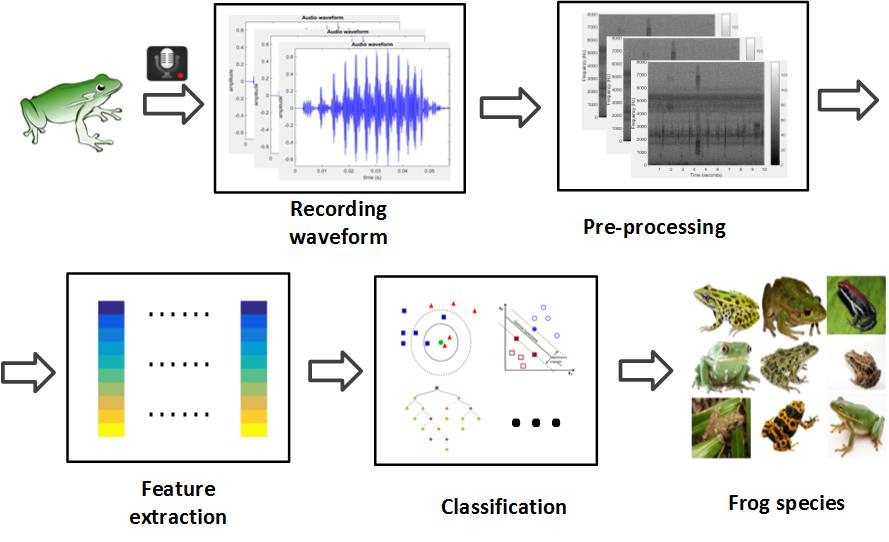
\includegraphics[width=\textwidth]{image/Ch1/flowchart.jpg}
%\caption[Flowchart of a frog call classification system]{Flowchart of a frog call classification system}
%\label{fig:Ch1_flowchart}
%\end{figure}
%
%
%\section{Research Challenges}
%Most datasets used in previous frog call classification studies assume that there is only one frog species in each individual recording. However, these resulting frog calls cannot reflect the characteristics of frog vocalisations in real-world situations, such as background noise, frog chorus, and other vocalising animals. To develop a robust frog call classification system for environmental recordings, two main challenges have been identified. 
%
%
%\noindent \textbf{Challenge 1}: Most previous work studied frog call classification using high SNR recordings, but the classification performance of different studies varied a lot with a relatively low classification accuracy. The first challenge of this thesis is to build an enhanced feature set to further improve the classification performance using high SNR recordings. 
%
%\noindent \textbf{Challenge 2}: Since our work finally aims to classify frog calls in low SNR recordings, most features that can successfully classify high SNR recordings will probably not perform well for low SNR recordings. Consequently, it is still a big challenge to develop robust acoustic features to classify frog species in low SNR recordings. 
%
%\noindent \textbf{Challenge 3}: Since most previous work assumed that each individual recording consists of only one frog species, a single-instance single-label (SISL) framework is suitable for classifying frog calls in those high SNR recordings Figure~\ref{fig:label}. However, as low SNR recordings often have different characteristics containing more than one frog species, the SISL framework is no longer suitable. Therefore, the last challenge of this thesis is to design a novel classification framework for studying frog vocalisations in low SNR recordings with overlapping vocalising frog species. 
%
%

%
%\section{Research questions}
%The research questions are developed in order to solve the aforementioned challenges, which can be categorised into three parts. 
%
%\begin{enumerate}
% \item How to improve the classification performance when addressing high SNR recordings?
% 
%\item How to develop robust acoustic features to classify frog calls in low SNR recordings?
%
%\item How to employ suitable classification frameworks to classify multiple simultaneous vocalising frog species in low SNR recordings?
% 
%\end{enumerate}
%
%
%
%
%\section{Aims and objectives}
%This thesis aims to investigate techniques for robust and effective classification of frog species in acoustic data for environmental monitoring. For high SNR recordings, we need to improve the classification performance. As for the low SNR recordings, we plan to design novel frameworks to classify multiple simultaneously vocalising frog species. With our classification results, ecologists can then make decisions on how to protect and improve the health of frog populations. The specific research objectives are listed below.
%
%
%\begin{enumerate}
%
%\item	To improve the current representation schemes for modelling frog calls in high SNR recordings
%
%\item 	To develop robust feature extraction methods for frog call classification in low SNR recordings 
%
%\item   To investigate machine learning techniques (multiple-instance multiple-label (MIML) learning and multiple-label (ML) learning) to tackle the frog call classification problem in low SNR recordings
%
%\end{enumerate}
% 
% 
% 
%\section{Significance and contributions}
%Due to the development of sensor techniques, acoustic sensors have been widely deployed in the field for surveying vocalising animals. Different from recordings collected in the constrained environment, recordings collected in the field often have a low SNR and contain multiple simultaneous vocalising frog species. In this dissertation, the performance of classifying frog species in high SNR recordings is investigated to be further improved.
%Then, features that can be used for studying frog calls in high SNR recordings are developed or adapted for analysing low SNR recordings.
%Since field recordings often consist of multiple simultaneous vocalising frog species, both MIML and ML learning are used for the classification of frog species in low SNR field recordings. Meanwhile, both frog calling activity and species can be monitored over long-term using our proposed classification framework.
%Further more, ecologists can monitor frogs by collecting audio data with the developed frog call classification framework, which will enable frog monitoring over large areas and long periods of time, and significantly reduce the expert labour cost for monitoring frog calling activity of a particular area. The monitoring results can also help reveal the importance of environmental protection, which can be achieved via studying the correlation between the frog calling activity/species richness and weather variables. 
%
%Below is a list of the publications arising from this PhD research.

%\begin{center}
%{\huge \textbf{List of Publications}}
%\end{center}





 
% 
%\section{Thesis structure} 
 






